% figures/cumulative_kl.tex -- Cumulative KL curves for IOI (5-prompt average)
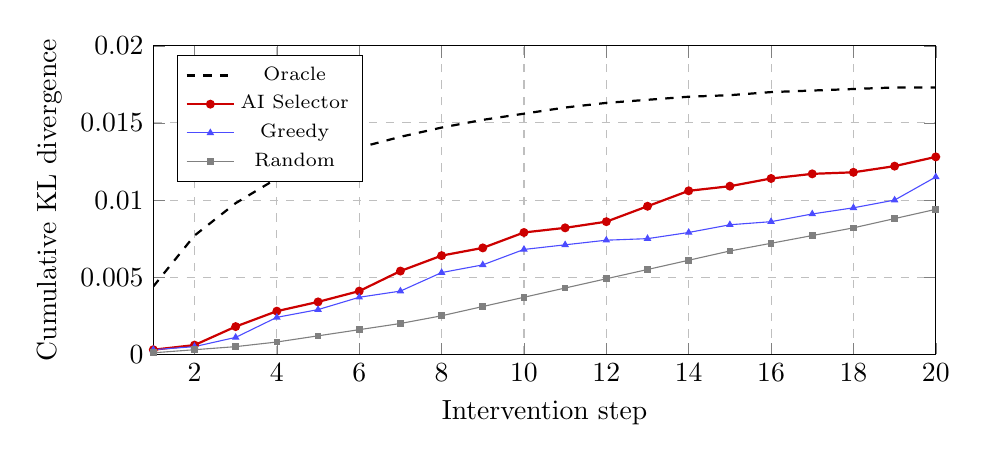
\begin{tikzpicture}
\begin{axis}[
    width=0.95\columnwidth,
    height=5.5cm,
    xlabel={Intervention step},
    ylabel={Cumulative KL divergence},
    xmin=1, xmax=20,
    ymin=0, ymax=0.020,
    legend pos=north west,
    legend style={font=\scriptsize},
    grid=major,
    grid style=dashed,
    scaled y ticks=false,
    yticklabel style={/pgf/number format/fixed, /pgf/number format/precision=3},
]

% Oracle (upper bound)
\addplot[color=black, dashed, thick] coordinates {
    (1, 0.0044) (2, 0.0077) (3, 0.0098) (4, 0.0114)
    (5, 0.0126) (6, 0.0134) (7, 0.0141) (8, 0.0147)
    (9, 0.0152) (10, 0.0156) (11, 0.0160) (12, 0.0163)
    (13, 0.0165) (14, 0.0167) (15, 0.0168) (16, 0.0170)
    (17, 0.0171) (18, 0.0172) (19, 0.0173) (20, 0.0173)
};
\addlegendentry{Oracle}

% AI Selector
\addplot[color=red!80!black, thick, mark=*, mark size=1.2pt] coordinates {
    (1, 0.0003) (2, 0.0006) (3, 0.0018) (4, 0.0028)
    (5, 0.0034) (6, 0.0041) (7, 0.0054) (8, 0.0064)
    (9, 0.0069) (10, 0.0079) (11, 0.0082) (12, 0.0086)
    (13, 0.0096) (14, 0.0106) (15, 0.0109) (16, 0.0114)
    (17, 0.0117) (18, 0.0118) (19, 0.0122) (20, 0.0128)
};
\addlegendentry{AI Selector}

% Greedy
\addplot[color=blue!70, mark=triangle*, mark size=1.2pt] coordinates {
    (1, 0.0003) (2, 0.0005) (3, 0.0011) (4, 0.0024)
    (5, 0.0029) (6, 0.0037) (7, 0.0041) (8, 0.0053)
    (9, 0.0058) (10, 0.0068) (11, 0.0071) (12, 0.0074)
    (13, 0.0075) (14, 0.0079) (15, 0.0084) (16, 0.0086)
    (17, 0.0091) (18, 0.0095) (19, 0.0100) (20, 0.0115)
};
\addlegendentry{Greedy}

% Random
\addplot[color=gray, mark=square*, mark size=1.0pt] coordinates {
    (1, 0.0001) (2, 0.0003) (3, 0.0005) (4, 0.0008)
    (5, 0.0012) (6, 0.0016) (7, 0.0020) (8, 0.0025)
    (9, 0.0031) (10, 0.0037) (11, 0.0043) (12, 0.0049)
    (13, 0.0055) (14, 0.0061) (15, 0.0067) (16, 0.0072)
    (17, 0.0077) (18, 0.0082) (19, 0.0088) (20, 0.0094)
};
\addlegendentry{Random}

\end{axis}
\end{tikzpicture}
